% Created by tikzDevice version 0.12.6 on 2024-07-30 15:54:53
% !TEX encoding = UTF-8 Unicode
  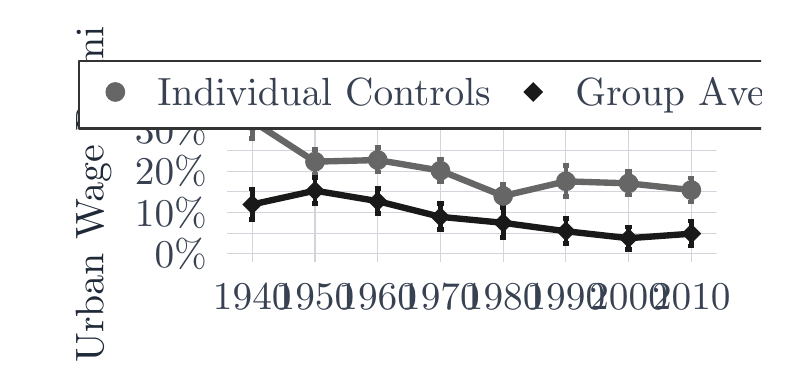
\begin{tikzpicture}[x=1pt,y=1pt]
  \definecolor{fillColor}{RGB}{255,255,255}
  \path[use as bounding box,fill=fillColor] (0,0) rectangle (264.99,120.45);
  \begin{scope}
  \path[clip] (  0.00,  0.00) rectangle (264.99,120.45);
  \definecolor{drawColor}{RGB}{255,255,255}

  \path[draw=drawColor,line width= 0.8pt,line join=round,line cap=round,fill=fillColor] (  0.00,  0.00) rectangle (264.99,120.45);
  \end{scope}
  \begin{scope}
  \path[clip] ( 71.98, 35.76) rectangle (248.99,104.45);
  \definecolor{drawColor}{RGB}{255,255,255}
  \definecolor{fillColor}{RGB}{255,255,255}

  \path[draw=drawColor,line width= 0.8pt,line join=round,line cap=round,fill=fillColor] ( 71.98, 35.76) rectangle (248.99,104.45);
  \definecolor{drawColor}{RGB}{209,213,219}

  \path[draw=drawColor,line width= 0.4pt,line join=round] ( 71.98, 46.21) --
    (248.99, 46.21);

  \path[draw=drawColor,line width= 0.4pt,line join=round] ( 71.98, 61.14) --
    (248.99, 61.14);

  \path[draw=drawColor,line width= 0.4pt,line join=round] ( 71.98, 76.08) --
    (248.99, 76.08);

  \path[draw=drawColor,line width= 0.4pt,line join=round] ( 71.98, 91.01) --
    (248.99, 91.01);

  \path[draw=drawColor,line width= 0.4pt,line join=round] ( 71.98, 38.74) --
    (248.99, 38.74);

  \path[draw=drawColor,line width= 0.4pt,line join=round] ( 71.98, 53.68) --
    (248.99, 53.68);

  \path[draw=drawColor,line width= 0.4pt,line join=round] ( 71.98, 68.61) --
    (248.99, 68.61);

  \path[draw=drawColor,line width= 0.4pt,line join=round] ( 71.98, 83.54) --
    (248.99, 83.54);

  \path[draw=drawColor,line width= 0.4pt,line join=round] ( 71.98, 98.48) --
    (248.99, 98.48);

  \path[draw=drawColor,line width= 0.4pt,line join=round] ( 81.16, 35.76) --
    ( 81.16,104.45);

  \path[draw=drawColor,line width= 0.4pt,line join=round] (103.82, 35.76) --
    (103.82,104.45);

  \path[draw=drawColor,line width= 0.4pt,line join=round] (126.49, 35.76) --
    (126.49,104.45);

  \path[draw=drawColor,line width= 0.4pt,line join=round] (149.15, 35.76) --
    (149.15,104.45);

  \path[draw=drawColor,line width= 0.4pt,line join=round] (171.82, 35.76) --
    (171.82,104.45);

  \path[draw=drawColor,line width= 0.4pt,line join=round] (194.48, 35.76) --
    (194.48,104.45);

  \path[draw=drawColor,line width= 0.4pt,line join=round] (217.15, 35.76) --
    (217.15,104.45);

  \path[draw=drawColor,line width= 0.4pt,line join=round] (239.81, 35.76) --
    (239.81,104.45);
  \definecolor{drawColor}{gray}{0.40}

  \path[draw=drawColor,line width= 2.3pt,line join=round] ( 81.16, 86.72) --
    (103.82, 72.03) --
    (126.49, 72.62) --
    (149.15, 68.79) --
    (171.82, 59.64) --
    (194.48, 64.92) --
    (217.15, 64.20) --
    (239.81, 61.76);
  \definecolor{drawColor}{gray}{0.10}

  \path[draw=drawColor,line width= 2.3pt,line join=round] ( 81.16, 56.57) --
    (103.82, 61.55) --
    (126.49, 57.76) --
    (149.15, 52.09) --
    (171.82, 49.93) --
    (194.48, 46.89) --
    (217.15, 44.37) --
    (239.81, 46.00);
  \definecolor{drawColor}{gray}{0.40}

  \path[draw=drawColor,line width= 1.7pt,line join=round] ( 80.03, 93.30) --
    ( 82.29, 93.30);

  \path[draw=drawColor,line width= 1.7pt,line join=round] ( 81.16, 93.30) --
    ( 81.16, 80.35);

  \path[draw=drawColor,line width= 1.7pt,line join=round] ( 80.03, 80.35) --
    ( 82.29, 80.35);
  \definecolor{drawColor}{gray}{0.10}

  \path[draw=drawColor,line width= 1.7pt,line join=round] ( 80.03, 62.16) --
    ( 82.29, 62.16);

  \path[draw=drawColor,line width= 1.7pt,line join=round] ( 81.16, 62.16) --
    ( 81.16, 51.17);

  \path[draw=drawColor,line width= 1.7pt,line join=round] ( 80.03, 51.17) --
    ( 82.29, 51.17);
  \definecolor{drawColor}{gray}{0.40}

  \path[draw=drawColor,line width= 1.7pt,line join=round] (102.69, 76.55) --
    (104.96, 76.55);

  \path[draw=drawColor,line width= 1.7pt,line join=round] (103.82, 76.55) --
    (103.82, 67.62);

  \path[draw=drawColor,line width= 1.7pt,line join=round] (102.69, 67.62) --
    (104.96, 67.62);
  \definecolor{drawColor}{gray}{0.10}

  \path[draw=drawColor,line width= 1.7pt,line join=round] (102.69, 66.42) --
    (104.96, 66.42);

  \path[draw=drawColor,line width= 1.7pt,line join=round] (103.82, 66.42) --
    (103.82, 56.82);

  \path[draw=drawColor,line width= 1.7pt,line join=round] (102.69, 56.82) --
    (104.96, 56.82);
  \definecolor{drawColor}{gray}{0.40}

  \path[draw=drawColor,line width= 1.7pt,line join=round] (125.36, 77.09) --
    (127.62, 77.09);

  \path[draw=drawColor,line width= 1.7pt,line join=round] (126.49, 77.09) --
    (126.49, 68.27);

  \path[draw=drawColor,line width= 1.7pt,line join=round] (125.36, 68.27) --
    (127.62, 68.27);
  \definecolor{drawColor}{gray}{0.10}

  \path[draw=drawColor,line width= 1.7pt,line join=round] (125.36, 62.39) --
    (127.62, 62.39);

  \path[draw=drawColor,line width= 1.7pt,line join=round] (126.49, 62.39) --
    (126.49, 53.26);

  \path[draw=drawColor,line width= 1.7pt,line join=round] (125.36, 53.26) --
    (127.62, 53.26);
  \definecolor{drawColor}{gray}{0.40}

  \path[draw=drawColor,line width= 1.7pt,line join=round] (148.02, 73.01) --
    (150.29, 73.01);

  \path[draw=drawColor,line width= 1.7pt,line join=round] (149.15, 73.01) --
    (149.15, 64.66);

  \path[draw=drawColor,line width= 1.7pt,line join=round] (148.02, 64.66) --
    (150.29, 64.66);
  \definecolor{drawColor}{gray}{0.10}

  \path[draw=drawColor,line width= 1.7pt,line join=round] (148.02, 56.88) --
    (150.29, 56.88);

  \path[draw=drawColor,line width= 1.7pt,line join=round] (149.15, 56.88) --
    (149.15, 47.43);

  \path[draw=drawColor,line width= 1.7pt,line join=round] (148.02, 47.43) --
    (150.29, 47.43);
  \definecolor{drawColor}{gray}{0.40}

  \path[draw=drawColor,line width= 1.7pt,line join=round] (170.68, 63.82) --
    (172.95, 63.82);

  \path[draw=drawColor,line width= 1.7pt,line join=round] (171.82, 63.82) --
    (171.82, 55.56);

  \path[draw=drawColor,line width= 1.7pt,line join=round] (170.68, 55.56) --
    (172.95, 55.56);
  \definecolor{drawColor}{gray}{0.10}

  \path[draw=drawColor,line width= 1.7pt,line join=round] (170.68, 55.45) --
    (172.95, 55.45);

  \path[draw=drawColor,line width= 1.7pt,line join=round] (171.82, 55.45) --
    (171.82, 44.60);

  \path[draw=drawColor,line width= 1.7pt,line join=round] (170.68, 44.60) --
    (172.95, 44.60);
  \definecolor{drawColor}{gray}{0.40}

  \path[draw=drawColor,line width= 1.7pt,line join=round] (193.35, 70.60) --
    (195.62, 70.60);

  \path[draw=drawColor,line width= 1.7pt,line join=round] (194.48, 70.60) --
    (194.48, 59.43);

  \path[draw=drawColor,line width= 1.7pt,line join=round] (193.35, 59.43) --
    (195.62, 59.43);
  \definecolor{drawColor}{gray}{0.10}

  \path[draw=drawColor,line width= 1.7pt,line join=round] (193.35, 51.52) --
    (195.62, 51.52);

  \path[draw=drawColor,line width= 1.7pt,line join=round] (194.48, 51.52) --
    (194.48, 42.40);

  \path[draw=drawColor,line width= 1.7pt,line join=round] (193.35, 42.40) --
    (195.62, 42.40);
  \definecolor{drawColor}{gray}{0.40}

  \path[draw=drawColor,line width= 1.7pt,line join=round] (216.01, 68.53) --
    (218.28, 68.53);

  \path[draw=drawColor,line width= 1.7pt,line join=round] (217.15, 68.53) --
    (217.15, 59.98);

  \path[draw=drawColor,line width= 1.7pt,line join=round] (216.01, 59.98) --
    (218.28, 59.98);
  \definecolor{drawColor}{gray}{0.10}

  \path[draw=drawColor,line width= 1.7pt,line join=round] (216.01, 48.44) --
    (218.28, 48.44);

  \path[draw=drawColor,line width= 1.7pt,line join=round] (217.15, 48.44) --
    (217.15, 40.40);

  \path[draw=drawColor,line width= 1.7pt,line join=round] (216.01, 40.40) --
    (218.28, 40.40);
  \definecolor{drawColor}{gray}{0.40}

  \path[draw=drawColor,line width= 1.7pt,line join=round] (238.68, 66.17) --
    (240.94, 66.17);

  \path[draw=drawColor,line width= 1.7pt,line join=round] (239.81, 66.17) --
    (239.81, 57.47);

  \path[draw=drawColor,line width= 1.7pt,line join=round] (238.68, 57.47) --
    (240.94, 57.47);
  \definecolor{drawColor}{gray}{0.10}

  \path[draw=drawColor,line width= 1.7pt,line join=round] (238.68, 50.61) --
    (240.94, 50.61);

  \path[draw=drawColor,line width= 1.7pt,line join=round] (239.81, 50.61) --
    (239.81, 41.52);

  \path[draw=drawColor,line width= 1.7pt,line join=round] (238.68, 41.52) --
    (240.94, 41.52);
  \definecolor{fillColor}{gray}{0.40}

  \path[fill=fillColor] ( 81.16, 86.72) circle (  3.57);
  \definecolor{fillColor}{gray}{0.10}

  \path[fill=fillColor] ( 77.59, 56.57) --
    ( 81.16, 60.14) --
    ( 84.73, 56.57) --
    ( 81.16, 53.00) --
    cycle;
  \definecolor{fillColor}{gray}{0.40}

  \path[fill=fillColor] (103.82, 72.03) circle (  3.57);
  \definecolor{fillColor}{gray}{0.10}

  \path[fill=fillColor] (100.26, 61.55) --
    (103.82, 65.12) --
    (107.39, 61.55) --
    (103.82, 57.98) --
    cycle;
  \definecolor{fillColor}{gray}{0.40}

  \path[fill=fillColor] (126.49, 72.62) circle (  3.57);
  \definecolor{fillColor}{gray}{0.10}

  \path[fill=fillColor] (122.92, 57.76) --
    (126.49, 61.33) --
    (130.06, 57.76) --
    (126.49, 54.19) --
    cycle;
  \definecolor{fillColor}{gray}{0.40}

  \path[fill=fillColor] (149.15, 68.79) circle (  3.57);
  \definecolor{fillColor}{gray}{0.10}

  \path[fill=fillColor] (145.58, 52.09) --
    (149.15, 55.65) --
    (152.72, 52.09) --
    (149.15, 48.52) --
    cycle;
  \definecolor{fillColor}{gray}{0.40}

  \path[fill=fillColor] (171.82, 59.64) circle (  3.57);
  \definecolor{fillColor}{gray}{0.10}

  \path[fill=fillColor] (168.25, 49.93) --
    (171.82, 53.50) --
    (175.39, 49.93) --
    (171.82, 46.37) --
    cycle;
  \definecolor{fillColor}{gray}{0.40}

  \path[fill=fillColor] (194.48, 64.92) circle (  3.57);
  \definecolor{fillColor}{gray}{0.10}

  \path[fill=fillColor] (190.91, 46.89) --
    (194.48, 50.46) --
    (198.05, 46.89) --
    (194.48, 43.32) --
    cycle;
  \definecolor{fillColor}{gray}{0.40}

  \path[fill=fillColor] (217.15, 64.20) circle (  3.57);
  \definecolor{fillColor}{gray}{0.10}

  \path[fill=fillColor] (213.58, 44.37) --
    (217.15, 47.94) --
    (220.72, 44.37) --
    (217.15, 40.80) --
    cycle;
  \definecolor{fillColor}{gray}{0.40}

  \path[fill=fillColor] (239.81, 61.76) circle (  3.57);
  \definecolor{fillColor}{gray}{0.10}

  \path[fill=fillColor] (236.24, 46.00) --
    (239.81, 49.57) --
    (243.38, 46.00) --
    (239.81, 42.43) --
    cycle;
  \end{scope}
  \begin{scope}
  \path[clip] (  0.00,  0.00) rectangle (264.99,120.45);
  \definecolor{drawColor}{RGB}{55,65,81}

  \node[text=drawColor,anchor=base east,inner sep=0pt, outer sep=0pt, scale=  1.42] at ( 64.78, 33.85) {0\%};

  \node[text=drawColor,anchor=base east,inner sep=0pt, outer sep=0pt, scale=  1.42] at ( 64.78, 48.78) {10\%};

  \node[text=drawColor,anchor=base east,inner sep=0pt, outer sep=0pt, scale=  1.42] at ( 64.78, 63.71) {20\%};

  \node[text=drawColor,anchor=base east,inner sep=0pt, outer sep=0pt, scale=  1.42] at ( 64.78, 78.65) {30\%};

  \node[text=drawColor,anchor=base east,inner sep=0pt, outer sep=0pt, scale=  1.42] at ( 64.78, 93.58) {40\%};
  \end{scope}
  \begin{scope}
  \path[clip] (  0.00,  0.00) rectangle (264.99,120.45);
  \definecolor{drawColor}{RGB}{55,65,81}

  \node[text=drawColor,anchor=base,inner sep=0pt, outer sep=0pt, scale=  1.42] at ( 81.16, 18.76) {1940};

  \node[text=drawColor,anchor=base,inner sep=0pt, outer sep=0pt, scale=  1.42] at (103.82, 18.76) {1950};

  \node[text=drawColor,anchor=base,inner sep=0pt, outer sep=0pt, scale=  1.42] at (126.49, 18.76) {1960};

  \node[text=drawColor,anchor=base,inner sep=0pt, outer sep=0pt, scale=  1.42] at (149.15, 18.76) {1970};

  \node[text=drawColor,anchor=base,inner sep=0pt, outer sep=0pt, scale=  1.42] at (171.82, 18.76) {1980};

  \node[text=drawColor,anchor=base,inner sep=0pt, outer sep=0pt, scale=  1.42] at (194.48, 18.76) {1990};

  \node[text=drawColor,anchor=base,inner sep=0pt, outer sep=0pt, scale=  1.42] at (217.15, 18.76) {2000};

  \node[text=drawColor,anchor=base,inner sep=0pt, outer sep=0pt, scale=  1.42] at (239.81, 18.76) {2010};
  \end{scope}
  \begin{scope}
  \path[clip] (  0.00,  0.00) rectangle (264.99,120.45);
  \definecolor{drawColor}{RGB}{31,41,55}

  \node[text=drawColor,rotate= 90.00,anchor=base,inner sep=0pt, outer sep=0pt, scale=  1.44] at ( 27.32, 70.10) {Urban Wage Premium};
  \end{scope}
  \begin{scope}
  \path[clip] (  0.00,  0.00) rectangle (264.99,120.45);
  \definecolor{drawColor}{gray}{0.20}
  \definecolor{fillColor}{RGB}{255,255,255}

  \path[draw=drawColor,line width= 0.8pt,line join=round,line cap=round,fill=fillColor] ( 18.46, 83.98) rectangle (302.51,108.43);
  \end{scope}
  \begin{scope}
  \path[clip] (  0.00,  0.00) rectangle (264.99,120.45);
  \definecolor{drawColor}{RGB}{255,255,255}
  \definecolor{fillColor}{RGB}{255,255,255}

  \path[draw=drawColor,line width= 0.8pt,line join=round,line cap=round,fill=fillColor] ( 24.46, 89.98) rectangle ( 38.91,104.43);
  \end{scope}
  \begin{scope}
  \path[clip] (  0.00,  0.00) rectangle (264.99,120.45);
  \definecolor{fillColor}{gray}{0.40}

  \path[fill=fillColor] ( 31.68, 97.21) circle (  3.57);
  \end{scope}
  \begin{scope}
  \path[clip] (  0.00,  0.00) rectangle (264.99,120.45);
  \definecolor{drawColor}{RGB}{255,255,255}
  \definecolor{fillColor}{RGB}{255,255,255}

  \path[draw=drawColor,line width= 0.8pt,line join=round,line cap=round,fill=fillColor] (175.47, 89.98) rectangle (189.93,104.43);
  \end{scope}
  \begin{scope}
  \path[clip] (  0.00,  0.00) rectangle (264.99,120.45);
  \definecolor{fillColor}{gray}{0.10}

  \path[fill=fillColor] (179.13, 97.21) --
    (182.70,100.78) --
    (186.27, 97.21) --
    (182.70, 93.64) --
    cycle;
  \end{scope}
  \begin{scope}
  \path[clip] (  0.00,  0.00) rectangle (264.99,120.45);
  \definecolor{drawColor}{RGB}{55,65,81}

  \node[text=drawColor,anchor=base west,inner sep=0pt, outer sep=0pt, scale=  1.42] at ( 46.91, 92.31) {Individual Controls};
  \end{scope}
  \begin{scope}
  \path[clip] (  0.00,  0.00) rectangle (264.99,120.45);
  \definecolor{drawColor}{RGB}{55,65,81}

  \node[text=drawColor,anchor=base west,inner sep=0pt, outer sep=0pt, scale=  1.42] at (197.93, 92.31) {Group Averages};
  \end{scope}
  \end{tikzpicture}
